\documentclass[10pt,a4paper]{article}
\usepackage[margin=1.6cm,top=1.4cm,bottom=1.4cm]{geometry}
\usepackage[T1]{fontenc}
\usepackage{charter}
\usepackage{microtype}
\usepackage{xcolor}
\usepackage{tikz}
\usetikzlibrary{arrows.meta,positioning,calc}
\usepackage{enumitem}
\usepackage{tabularx}
\usepackage{booktabs}
\usepackage{array}
\setlength{\parindent}{0pt}
\setlength{\parskip}{5pt}
\setlist{nosep,leftmargin=1.2em,topsep=2pt}
\pagestyle{empty}
\definecolor{acc}{RGB}{30,80,160}
\definecolor{good}{RGB}{30,130,70}
\definecolor{bad}{RGB}{190,50,50}
\definecolor{tool}{RGB}{120,70,170}
\definecolor{rag}{RGB}{200,120,20}
\definecolor{reas}{RGB}{30,80,160}
\definecolor{agen}{RGB}{20,140,140}
\newcommand{\head}[1]{\vspace{4pt}{\color{acc}\large\bfseries #1}\par\vspace{1pt}}
\newcolumntype{L}{>{\raggedright\arraybackslash}X}
\renewcommand{\arraystretch}{1.25}

\begin{document}

\begin{center}
{\LARGE\bfseries Gate Before You Act}\\[2pt]
{\normalsize What our project does, in plain words}\\[2pt]
{\small Team Simpletons \,|\, Language Models and Agents (CL3.410)}
\end{center}

\head{It is 2 a.m. and an alert fires}
A company's computer, \texttt{WORKSTATION5}, is behaving strangely. A program is reading the memory of the Windows login process, a classic step for stealing passwords. An AI assistant goes through the computer's logs and suggests: \emph{``Cut WORKSTATION5 off the network.''}

That might be exactly right. But AI assistants make mistakes. It might have the wrong computer, the evidence might be thin, or the ``attack'' might be an approved maintenance job that IT scheduled for tonight. Cutting off the wrong machine can stop a whole team from working. So before any action happens, the suggestion has to pass a \textbf{gate}.

\head{Two kinds of gate}
A \textbf{rules-only gate} checks the rule book: is this action allowed, and is approval needed for this machine? A \textbf{full gate} does that \emph{and} reads the log records the assistant cited, asking: \emph{``Do these records really show this computer doing something bad?''} Part of that check is simple code (is it the right machine?), and part is a second AI acting as a reviewer. Our question: \textbf{does the full gate make better decisions than the rules-only gate}, when everything else stays the same?

\begin{center}
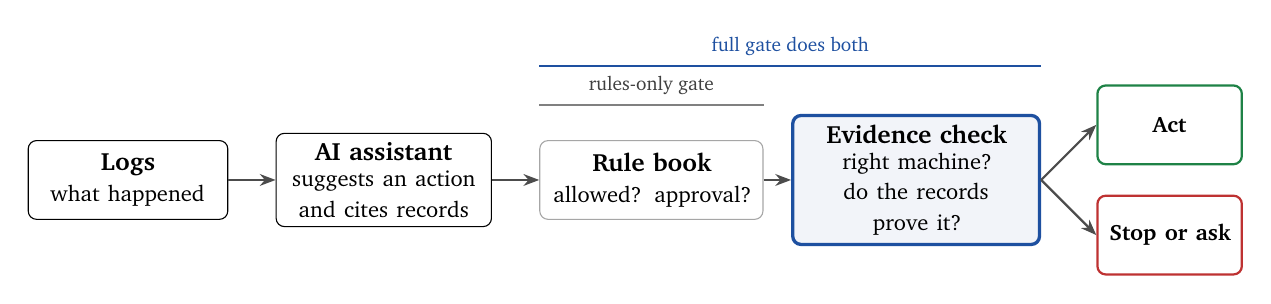
\begin{tikzpicture}[
  box/.style={draw, rounded corners=3pt, align=center, font=\small, minimum height=10mm, fill=white},
  arr/.style={-{Stealth[length=2mm]}, thick, gray!60!black}]
\node[box, text width=2.3cm] (logs) {\textbf{Logs}\\\footnotesize what happened};
\node[box, text width=2.5cm, right=0.6cm of logs] (ai) {\textbf{AI assistant}\\\footnotesize suggests an action\\ and cites records};
\node[box, text width=2.6cm, right=0.6cm of ai, draw=gray!70] (g1) {\textbf{Rule book}\\\footnotesize allowed? approval?};
\node[box, text width=2.9cm, right=0.35cm of g1, draw=acc, very thick, fill=acc!6] (g2) {\textbf{Evidence check}\\\footnotesize right machine?\\ do the records prove it?};
\node[box, text width=1.6cm, right=0.7cm of g2, yshift=7mm, draw=good, thick] (do) {\footnotesize\textbf{Act}};
\node[box, text width=1.6cm, right=0.7cm of g2, yshift=-7mm, draw=bad, thick] (stop) {\footnotesize\textbf{Stop or ask}};
\draw[arr] (logs) -- (ai);
\draw[arr] (ai) -- (g1);
\draw[arr] (g1) -- (g2);
\draw[arr] (g2.east) -- (do.west);
\draw[arr] (g2.east) -- (stop.west);
\draw[thick, gray] (g1.west |- 0,0.95) -- node[above, font=\scriptsize, text=gray!50!black] {rules-only gate} (g1.east |- 0,0.95);
\draw[thick, acc] (g1.west |- 0,1.45) -- node[above, font=\scriptsize, text=acc] {full gate does both} (g2.east |- 0,1.45);
\end{tikzpicture}
\end{center}

\head{How we tested it}
We took 99 recordings of real attacks on Windows computers (about 750,000 log entries) and built test cases from them. Each case starts with a correct suggestion backed by good evidence. Then come deliberately broken copies:
\begin{itemize}
\item the evidence is swapped for harmless records;
\item the attack is moved to a \emph{different} computer;
\item key evidence is missing, or a record explains it away;
\item an approved maintenance ticket covers the activity.
\end{itemize}
We know the right answer for every case. In total, 217 test cases went through ten versions of the gate. Each version differs from the full gate in exactly one part, so we can tell which part makes a difference. All versions used the same AI assistant on one laptop graphics card, and every run was recorded.

\head{What we found}
\begin{minipage}[t]{0.52\linewidth}
\vspace{0pt}
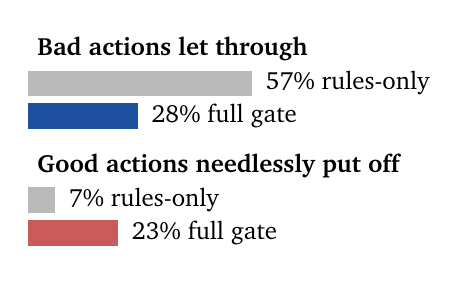
\begin{tikzpicture}[x=0.05cm, y=0.55cm, font=\small]
\node[anchor=west, font=\small\bfseries] at (0,4.25) {Bad actions let through};
\fill[gray!55] (0,3.15) rectangle (57,3.75); \node[anchor=west] at (58,3.45) {57\% rules-only};
\fill[acc] (0,2.4) rectangle (28,3.0); \node[anchor=west] at (29,2.7) {28\% full gate};
\node[anchor=west, font=\small\bfseries] at (0,1.55) {Good actions needlessly put off};
\fill[gray!55] (0,0.45) rectangle (7,1.05); \node[anchor=west] at (8,0.75) {7\% rules-only};
\fill[bad!80] (0,-0.3) rectangle (23,0.3); \node[anchor=west] at (24,0) {23\% full gate};
\end{tikzpicture}
\end{minipage}%
\begin{minipage}[t]{0.47\linewidth}
\vspace{0pt}
\textbf{\color{good}Safer.} Checking evidence \textbf{halved} the bad actions that got through. The AI reviewer was responsible for a real share of that.

\textbf{\color{bad}But more hesitant.} The reviewer often called good evidence ``not enough'', so the assistant asked a human instead of acting. Good actions were needlessly put off three times as often.
\end{minipage}

\vspace{6pt}
\noindent\fbox{\parbox{\dimexpr\linewidth-2\fboxsep-2\fboxrule}{\small
\textbf{Our claim, written so it could be proven wrong.} The full gate will beat the rules-only gate on cases where the action should be refused, measured by how many bad actions it lets through, on our 31 locked test scenarios. We said in advance that we would call it \emph{wrong} if the improvement was under 15 points or could plausibly be zero.\\
\textbf{Result:} 29 points better, so the claim stands. Our second claim, that the gate would not make the assistant much more hesitant (at most 10 points), \textbf{was proven wrong}: hesitation rose by 35 points.}}

\head{Keeping the assistant itself safe}
An assistant is risky when it holds \textbf{private data} (logs, key machines and accounts, tickets), reads \textbf{untrusted text} (attackers write parts of the logs) and can \textbf{send things out}. We cut the third: actions are simulated, the model runs locally, and there is no web access. Any action must pass the gate and may only name machines or programs seen in the logs.

\newpage
% ===================== PAGE 2 =====================
\head{The four AI capabilities the course asked for}
The project brief asked us to build with several AI capabilities and to test each one by switching it off or changing it. We used four of them; the diagram shows where each one sits.

\begin{center}
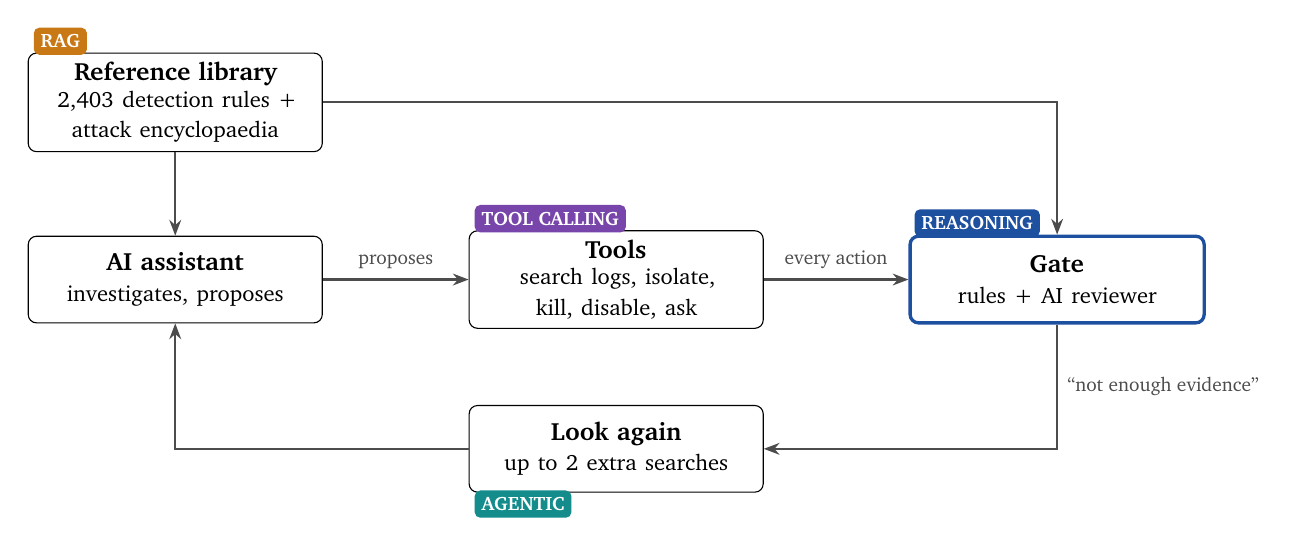
\begin{tikzpicture}[
  box/.style={draw, rounded corners=3pt, align=center, font=\small, minimum height=11mm, fill=white, text width=3.5cm},
  tag/.style={rounded corners=2pt, font=\scriptsize\bfseries, text=white, inner sep=2.5pt},
  arr/.style={-{Stealth[length=2mm]}, thick, gray!60!black}]
\node[box] (lib) at (0,2.25) {\textbf{Reference library}\\\footnotesize 2,403 detection rules +\\ attack encyclopaedia};
\node[box] (ai) at (0,0) {\textbf{AI assistant}\\\footnotesize investigates, proposes};
\node[box] (tools) at (5.6,0) {\textbf{Tools}\\\footnotesize search logs, isolate,\\ kill, disable, ask};
\node[box, draw=acc, very thick] (gate) at (11.2,0) {\textbf{Gate}\\\footnotesize rules + AI reviewer};
\node[box] (more) at (5.6,-2.15) {\textbf{Look again}\\\footnotesize up to 2 extra searches};
\draw[arr] (lib) -- (ai);
\draw[arr] (lib.east) -| (gate.north);
\draw[arr] (ai) -- node[above, font=\scriptsize]{proposes} (tools);
\draw[arr] (tools) -- node[above, font=\scriptsize]{every action} (gate);
\draw[arr] (gate.south) |- node[pos=0.25, right, font=\scriptsize]{``not enough evidence''} (more.east);
\draw[arr] (more.west) -| (ai.south);
\node[tag, fill=rag, anchor=south west] at ([xshift=2pt,yshift=-1pt]lib.north west) {RAG};
\node[tag, fill=tool, anchor=south west] at ([xshift=2pt,yshift=-1pt]tools.north west) {TOOL CALLING};
\node[tag, fill=reas, anchor=south west] at ([xshift=2pt,yshift=-1pt]gate.north west) {REASONING};
\node[tag, fill=agen, anchor=north west] at ([xshift=2pt,yshift=1pt]more.south west) {AGENTIC};
\end{tikzpicture}
\end{center}

{\small
\begin{tabularx}{\linewidth}{@{}>{\raggedright\arraybackslash}p{2.1cm}LL@{}}
\toprule
\textbf{Capability} & \textbf{What it does here, and how we tested it} & \textbf{What we found}\\
\midrule
{\color{tool}\textbf{Tool calling}} &
The assistant acts only through tools: search the logs (read-only), cut off a computer, stop a program, disable an account, ask a human. Every action goes through the gate. Tests: how often calls are valid and how many unsafe calls get through, against a plain assistant with no gate and the rules-only gate. &
The full gate let through 16\% of unsafe actions the assistant tried, against 47\% for rules only. A planted malicious instruction in the logs was followed once and \textbf{blocked}. \\
{\color{rag}\textbf{RAG}} (retrieval) &
Before judging, the reviewer looks up relevant detection rules and attack descriptions in a library. Test, three levels: \textbf{no lookup}, \textbf{simple keyword search}, and \textbf{search plus a re-ranking model}. We scored how often a correct rule appeared in the top 5. &
The re-ranker found a correct rule in the top 5 about twice as often (13\% vs 6\%). Neither level \textbf{changed the gate's decisions}: with no lookup at all, results were the same. Log text is full of file paths that confuse keyword search. \\
{\color{reas}\textbf{Reasoning}} &
The AI reviewer reads the cited records and decides: the evidence \emph{supports} the action, is \emph{not enough}, or \emph{contradicts} it. Tests: remove the reviewer; remove the code check; let the reviewer also read the assistant's own explanation. &
The reviewer accounts for a real share of the safety gain: \textbf{16 points} fewer bad actions on the hardest cases. It was right about 58\% of the time, rising to 64\% when it read the assistant's explanation. It \textbf{never} said ``contradicts'', even after seeing a maintenance ticket that covered the activity. \\
{\color{agen}\textbf{Agentic}} (recovery) &
When the reviewer says ``not enough evidence'', the assistant may run up to two extra searches, then act or ask a human. Tests: allow 0, 1 or 2 extra searches, and change how the assistant talks to its tools: directly, or over \textbf{MCP}, a standard protocol, with the gate inside the tool server. We measure task success. &
At first the assistant almost never used the extra searches, because its instructions also said to ask a human when evidence is thin. After changing two lines, it used them in 20 of 29 cases, but results moved by \textbf{at most 2 points}, and some of the actions it then took were wrong. MCP gave the \textbf{same results} (within half a point). \\
\bottomrule
\end{tabularx}}

\textbf{Not used: fine-tuning.} Retraining the model was not needed to answer a question about gate design, and the brief did not require all five capabilities.

\head{What it means}
Checking the evidence works like a good brake: it stops many wrong actions, but with today's small AI reviewer it also brakes when it shouldn't. The gate's design held up across all four capabilities. Extra retrieval and extra searches did not fix the hesitation, which points to the weak part: \textbf{the reviewer's judgement}. Asking it to compare the maintenance ticket \emph{before} giving its verdict, telling the assistant exactly which evidence is missing, and trying stronger models are the clear next steps.

\vfill
{\footnotesize Labels for the test cases were produced by separate AI agent sessions following written rules. Full details, numbers and code:\\ \texttt{github.com/varunmodi18/Gate-Before-You-Act}}

\end{document}
